% 2008 年上海卷理科第 17 题：圆心角 120° 的扇形 AOB，出入口在 A、C，
%   小路 CD∥BO，D 在 OA 上，CD=500 m，DA=300 m，求半径 OA。
% 来源 PDF：gaokaomath-src/普通高考/2008/2008上海理.pdf
% SHA-256：df3f761eb2551cc795c0efb1c90c284a54b95265e327f21abb60aa0f4bdd86a2
% 原页：2008上海理.pdf 第 1 页（A3 三栏）第 3 栏，书页码 479。
% 重绘依据：按 R=1 归一化，A 在 150°、B 在 30°，OD/R=145/445.45≈0.326，
%   CD/R=500/445.45≈1.123，C=(0.690,0.724) 落在单位圆上。
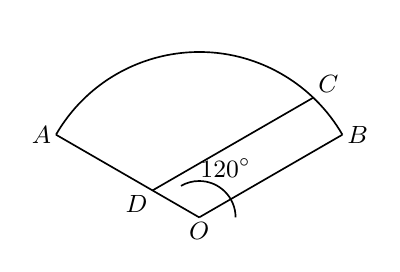
\begin{tikzpicture}[scale=2.1, semithick,
  every node/.style={inner sep=1.5pt}, font=\small]
  \coordinate (O) at (0,0);
  \coordinate (A) at (150:1);
  \coordinate (B) at (30:1);
  \coordinate (D) at (150:0.326);
  \coordinate (C) at (0.690,0.724);

  \draw (A) arc[start angle=150, end angle=30, radius=1];
  \draw (O) -- (A);
  \draw (O) -- (B);
  \draw (D) -- (C);

  \draw (0.22,0) arc[start angle=0, end angle=120, radius=0.22];
  \node at (0.16,0.30) {$120^\circ$};

  \node[left] at (A) {$A$};
  \node[right] at (B) {$B$};
  \node[above right] at (C) {$C$};
  \node[below left] at (D) {$D$};
  \node[below] at (O) {$O$};
\end{tikzpicture}
